
\serie{Autour du triangle}

\begin{exercice}
Recopie et complète les phrases en utilisant les mots « côté », « sommet », « triangle » et « opposé » : \\[-3em]
\begin{minipage}[c]{0.26\linewidth}
 \vspace{1.5cm}
 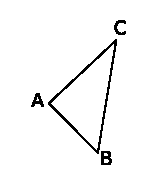
\includegraphics[width=1.8cm]{triangleCAB_vert}
 \end{minipage} \hfill%
 \begin{minipage}[t]{0.68\linewidth}
  \begin{enumerate}
   \item $ABC$ est un \ldots \ldots \ldots ;
   \item $[AB]$ est un  \ldots \ldots\ldots ;
   \item $C$ est un  \ldots \ldots\ldots ;
   \item $[BC]$ est  \ldots \ldots \ldots au sommet $A$ ;
   \item $B$ est le  \ldots \ldots \ldots au  \ldots \ldots \ldots $[AC]$ ;
   \end{enumerate}
 \end{minipage} \\
\end{exercice}


\begin{exercice}[Triangles particuliers]
 \begin{center} 
\includegraphics[width=2.5cm]{triangleGHI_rose} \qquad 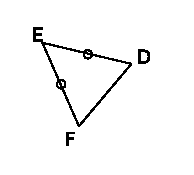
\includegraphics[width=2.4cm]{triangleEDF_brun} \end{center}
 Quelle est la nature du triangle $GHI$ ? Du triangle $DEF$ ? Justifie tes réponses.
\end{exercice}

\begin{exercice}[Avec le codage]
\begin{center} 
\includegraphics[width=3cm]{codage} \end{center}
\begin{enumerate}
 \item Quels sont les triangles équilatéraux ?
 \item Quels sont les triangles isocèles que l'on peut tracer en joignant des points de la figure ?
 \end{enumerate}
\end{exercice}

\begin{exercice}[Reconnaître]
Donne, en justifiant, la nature de chacun des triangles s'il est particulier :
\begin{colenumerate}{4}
 \item 
 
 
\includegraphics[width=1.2cm]{reconnaitre1}
 \item 
 
 
\includegraphics[width=1.3cm]{reconnaitre2}
 \item 
 
 
\includegraphics[width=1.6cm]{reconnaitre3}
 \item 
 
 
\includegraphics[width=1.4cm]{reconnaitre4}
 \end{colenumerate}
\end{exercice}

%%%%%%%%%%%%%%%%%%%%%%%%%%%%%%%%%%%%%%%%%%%%%%%%%%%%%%%%%%%%

\serie{Constructions}

\begin{exercice}
Indique si chacun des triangles donnés ci-dessous est constructible ou non :

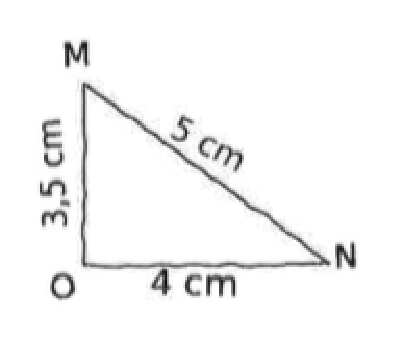
\includegraphics[width=2cm]{triangleMON} \hfill 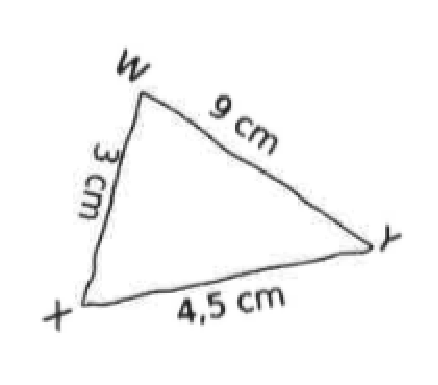
\includegraphics[width=2cm]{triangleWYX} \hfill 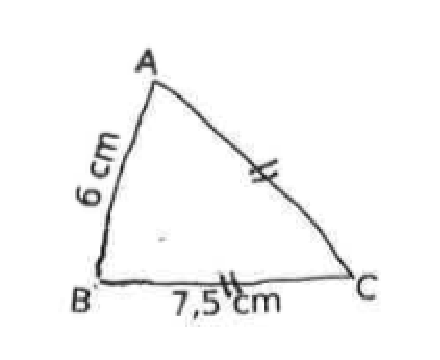
\includegraphics[width=2cm]{triangleBCA}
\end{exercice}


\begin{exercice}
Explique pourquoi il est impossible de construire de tels triangles :

\hfill 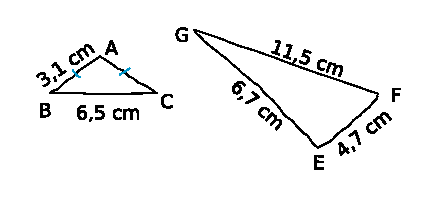
\includegraphics[width=5.7cm]{triangles_impos} \hfill 
\end{exercice}


\begin{exercice}
Construis les figures suivantes :

\hfill 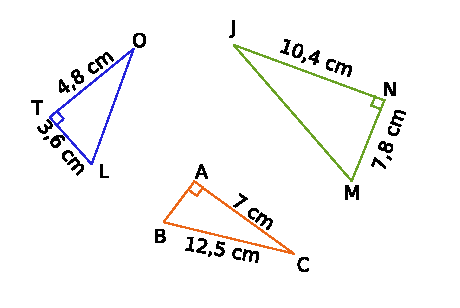
\includegraphics[width=6cm]{triangles_colores} \hfill 
\end{exercice}


\begin{exercice}
Dans chaque cas, effectue un croquis puis construis la figure.

 \begin{enumerate}
  \item Trace un triangle $FIN$ rectangle en $F$ tel que $FI = 5$ cm et $NF = 6$ cm ;
  \item Trace un triangle $TRS$ rectangle en $S$ tel que $TS = 72$ mm et $SR = 85$ mm ;
  \item Trace un triangle $GLU$ rectangle en $L$ tel que $LG = 8$ cm et $GU = 10$ cm.
  \end{enumerate}
\end{exercice}


\begin{exercice}[Construis \ldots]
 \begin{enumerate}
  \item Construis un triangle $MNO$ équilatéral de côté 5 cm ;
  \item Construis un triangle isocèle $STU$ isocèle en $S$ tel que $ST = 58$ mm et $TU = 32$ mm ;
  \item Construis un triangle $ABC$ tel que $AB = 6$ cm ; $BC = 5,2$ cm et $CA = 42$ mm.
  \end{enumerate}
\end{exercice}


\begin{exercice}
Quelle figure correspond au programme de construction suivant ? Justifie ta réponse.
 \begin{itemize}
  \item Construis un triangle $ABC$ rectangle en $A$ ;
  \item Construis $d_1$ la parallèle à $(BC)$ passant par $A$ ;
  \item Construis $d_2$ la médiatrice du segment $[AB]$ ;
  \item Place $D$ le point d'intersection des droites $d_1$ et $d_2$.
  \end{itemize}
  \begin{colenumerate}{2}
   \item 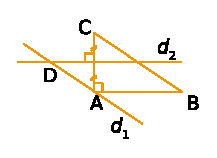
\includegraphics[width=2.9cm]{triangleCABD_1}
   \item 
\includegraphics[width=1.9cm]{triangleCABD_2}   
   \item 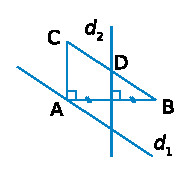
\includegraphics[width=2.5cm]{triangleCABD_3}
   \item 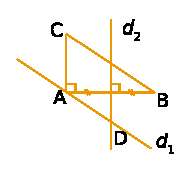
\includegraphics[width=2.6cm]{triangleCABD_4}
   \end{colenumerate}
\end{exercice}


\begin{exercice}[Demandez le programme]
Remets les consignes du programme de construction dans l'ordre :
\begin{center} 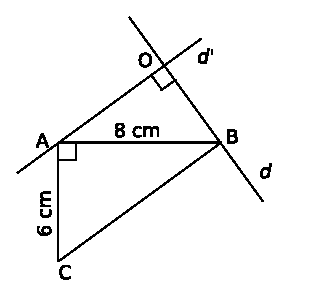
\includegraphics[width=4.1cm]{programme} \end{center}
 \begin{itemize}
  \item Trace la droite $d'$ parallèle à $(BC)$ passant par $A$ ;
  \item Nomme $O$ le point d'intersection de $d$ et $d'$ ;
  \item Trace un triangle $ABC$ rectangle en $A$, tel que $AB = 8$ cm et $AC = 6$ cm ;
  \item Trace la droite $d$ perpendiculaire à $d'$ et passant par $B$.
  \end{itemize}
\end{exercice}


\begin{exercice}[Triangle et losange]
 \begin{enumerate}
  \item Construis un triangle isocèle $ABC$ isocèle en $C$ tel que $AB = 3,5$ cm et $AC = 4,2$ cm ;
  \item Complète la figure avec la construction du point $D$ de sorte que $ACBD$ soit un losange ;
  \item Construis un triangle équilatéral $ABE$.
Qu'observes‑tu ?
   \end{enumerate}
\end{exercice}


\begin{exercice}
Trace un triangle $ABC$ isocèle en $A$ tel que $AB = 5$ cm et $BC = 3$ cm et un triangle $BCD$ isocèle en $D$ tel que $BD = 3,5$ cm.
\end{exercice}


\begin{exercice}[Le même triangle ?]
 \begin{enumerate}
  \item Trace un triangle $TRI$ tel que 
  
  $\widehat{TRI} = 45^\circ$ et  $\widehat{TIR} = 110^\circ$ ;
  \item Tes camarades obtiendront‑ils forcément un triangle identique au tien ?
  \end{enumerate}
\end{exercice}


\begin{exercice}
Dans chaque cas, effectue un croquis :
 \begin{enumerate}
  \item $SUR$ est un triangle tel que 
  
  $SU = 4,5$ cm, $\widehat{USR} = 60^\circ$ et $\widehat{RUS} = 40^\circ$ ;
  \item $QTD$ est un triangle tel que 
  
  $QT = 10$ cm, $TD = 7$ cm et $\widehat{QTD} = 70^\circ$ ;
  \item $MFV$ est un triangle tel que 
  
  $MF = 9$ cm, $FV = 12$ cm et $MV = 6$ cm.
  \end{enumerate}
\end{exercice}


\begin{exercice}[Reporter pour reproduire]
Reproduis les triangles suivants en utilisant uniquement une règle non graduée et un compas :
\begin{center} 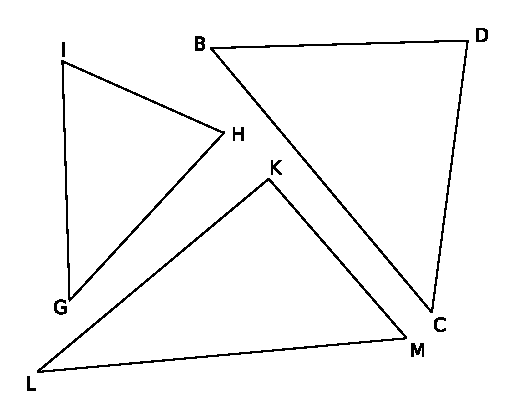
\includegraphics[width=7.1cm]{reproduire} \end{center}
\end{exercice}


\begin{exercice}
Après avoir effectué un croquis, construis les triangles suivants :
 \begin{enumerate}
  \item $GHI$ est un triangle tel que 
  
  $GH = 8$ cm, $HI = 5$ cm et $GI = 6$ cm ;
  \item $MNO$ est un triangle tel que 
  
  $MN = 4,5$ cm, $MO = 7$ cm et $\widehat{NMO} = 48^\circ$ ;
  \item $DEF$ est un triangle tel que 
  
  $DE = 8$ cm, $\widehat{FDE} = 45^\circ$ et $\widehat{FED} = 28^\circ$. 
  \end{enumerate}
\end{exercice}


\begin{exercice}
Dans chaque cas, effectue un croquis :
 \begin{enumerate}
  \item $POL$ est un triangle isocèle en $P$ tel que $PO = 14$ cm et $LO = 5$ cm ;
  \item $MER$ est un triangle équilatéral tel que $ME = 5$ cm ;
  \item $FAC$ est un triangle rectangle en $C$ tel que 
  
  $\widehat{AFC}= 50^\circ$ et $CA = 6,5$ cm.  
  \end{enumerate}
\end{exercice}


\begin{exercice}
Dans chaque cas, fais un croquis et construis :
 \begin{enumerate}
  \item $VUZ$ est un triangle isocèle en $U$ tel que 
  
  $VU = 6,5$ cm et $VZ = 4,5$ cm ;
  \item $KGB$ est un triangle équilatéral tel que 
  
  $KG = 6$ cm ;
  \item $CIA$ est un triangle rectangle en $C$ tel que $\widehat{CIA} = 37^\circ$ et $CI = 5,5$ cm ;
  \item $RTL$ est un triangle isocèle en $T$ tel que $RT = 8$ cm et $\widehat{TRL} = 48^\circ$.
  \end{enumerate}
\end{exercice}


\begin{exercice}
Sur ton cahier, reproduis en vraie grandeur la figure ci-dessous :
\begin{center} 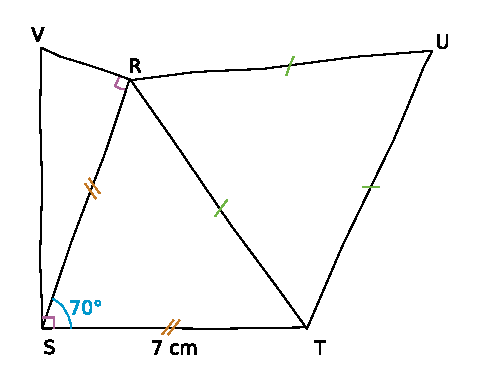
\includegraphics[width=6.9cm]{construction70} \end{center}
Écris ensuite le programme de construction.
\end{exercice}


\begin{exercice}
Dans chaque cas, fais un croquis et construis :
 \begin{enumerate}
  \item $EFG$ est un triangle tel que 
  
  $EF = 7,5$ cm, $\widehat{EFG} = 49^\circ$ et $\widehat{EGF} = 72^\circ$ ;
  \item $PLM$ est un triangle équilatéral de périmètre 15 cm ;
  \item Le triangle $RST$ est isocèle en $S$ de périmètre 13 cm et tel que $ST = 4$ cm ;
  \item Le triangle $AYB$ est isocèle et rectangle en $Y$ tel que $BA = 7$ cm ;
  \item Le triangle $OCI$ est isocèle en $I$ tel que $CO = 4,5$ cm et $\widehat{CIO} = 30^\circ$.
  \end{enumerate}
\end{exercice}


%%%%%%%%%%%%%%%%%%%%%%%%%%%%%%%%%%%%%%%%%%%%%%%%%%%%%%%%%%%%

\serie{Droites remarquables}

\begin{exercice}[Hauteurs d'un triangle]
Construis un triangle $BON$ tel que 

$BO = 68$ mm, $BN = 62$ mm et $NO = 45$ mm.

Trace :
\begin{itemize}
 \item En noir, la perpendiculaire à $(BN)$ passant par $O$ ;
 \item En rouge, la perpendiculaire à $(NO)$ passant par $B$ ;
 \item En vert, la perpendiculaire à $(BO)$ passant par $N$. Que remarques‑tu ?
 \end{itemize}
\end{exercice}


\begin{exercice}[Hauteur (« relative à » ou « issue de »)]
\begin{enumerate}
 \item Construis un triangle $AVE$ quelconque puis trace :
 \begin{itemize}
  \item En bleu, la hauteur issue du sommet $E$ ;
  \item En noir, la hauteur issue du sommet $A$ ;
  \item En rouge, la hauteur relative à $[AE]$.
  \end{itemize}
 \item Observe ces trois hauteurs. Quelle remarque peux-tu faire ?
 \end{enumerate}
\end{exercice}


\begin{exercice}[À l'intérieur ou pas ?]
\begin{enumerate}
 \item Construis un triangle $DER$ ayant tous ses angles aigus. Trace les hauteurs de ce triangle ;
 \item Construis un triangle $NRV$ tel que $\widehat{NRV}$ soit un angle obtus. Trace les hauteurs de ce triangle ;
 \item Construis un triangle $GHT$ rectangle en $T$. Trace les hauteurs de ce triangle ;
 \item Observe les trois figures. Quelles remarques peux-tu faire ?
 \end{enumerate}
\end{exercice}


\begin{exercice}[Médiatrices dans un triangle]
\begin{enumerate}
 \item Construis un triangle $ABC$ tel que $AB = 5,7$ cm, $AC = 5,3$ cm et $BC = 7$ cm.
 \item Construis les médiatrices des segments $[AB]$ et $[CB]$. Note $O$ leur point d'intersection.
 \item Construis la médiatrice du segment $[AC]$. Que constates‑tu ?
 \item Trace le cercle de centre $O$ passant par $A$. Comment s'appelle ce cercle ?
 \end{enumerate}
\end{exercice}


\begin{exercice}[Bissectrice dans un triangle]
\begin{enumerate}
 \item Trace un triangle $UST$ tel que 
 
 $UT = 3$ cm ; $US = 5$ cm et $ST = 7$ cm ;
 \item Construis les bissectrices des angles $\widehat{UST}$, $\widehat{UTS}$ et $\widehat{TUS}$.
 \end{enumerate}
 \vspace{-0.3cm}
Que constates‑tu ?
\end{exercice}


\begin{exercice}[Croquis et codages]
\begin{enumerate}
 \item Construis le triangle $TOC$ tel que 
 
 $TO = 8$ cm, $OC = 4,5$ cm et $CT = 6$ cm ;
 \item Trace puis code :
  \begin{itemize}
   \item En rouge, la hauteur issue de $O$ ;
   \item En bleu, la médiatrice de $[TO]$ ;
   \item En noir, la médiane relative à $[OC]$.
   \end{itemize} 
 \end{enumerate}
\end{exercice}


\begin{exercice}
Dans les 6 cas suivants :
\begin{colenumerate}{3}
 \item
 
 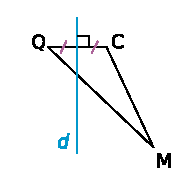
\includegraphics[width=2.3cm]{cas_1}
 \item
 
 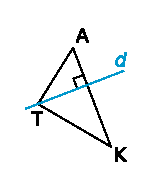
\includegraphics[width=1.6cm]{cas_2}
 \item
 
 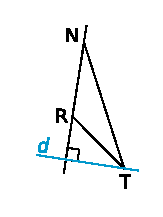
\includegraphics[width=1.7cm]{cas_3}
 \item
 
 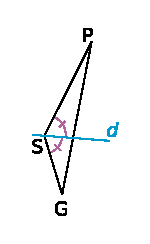
\includegraphics[width=1.6cm]{cas_4}
 \item
 
 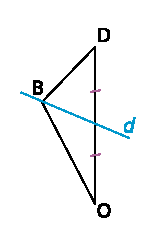
\includegraphics[width=1.8cm]{cas_5}
 \item
 
 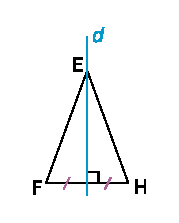
\includegraphics[width=1.8cm]{cas_6}
 \end{colenumerate}
Détermine dans quel(s) cas la droite $d$ est :
\begin{enumerate}
 \item Une hauteur ;
 \item Une médiatrice ;
 \item Une bissectrice ;
 \item Une médiane.
 \end{enumerate}
\end{exercice}


\begin{exercice}[Vocabulaire] \label{triangles_vocabulaire}
\begin{enumerate}
 \item Construis un triangle $BOA$ tel que $BO = 5$ cm, $OA = 7$ cm et $AB = 8$ cm. Trace la droite $d_1$ perpendiculaire à $[BO]$ et passant par $A$ ;
 \item Trace la droite $d_2$ perpendiculaire au segment $[OA]$ et passant par son milieu ;
 \item Trace la droite $d_3$ qui coupe l'angle $\widehat{OBA}$ en deux angles égaux ;
 \item Trace la droite $d_4$ qui passe par $O$ et par le milieu de $[BA]$ ;
 \item Détermine quelle(s) droite(s) représente(nt) une hauteur du triangle ;
 \item Détermine quelle(s) droite(s) représente(nt) une médiatrice ;
 \item Détermine quelle(s) droite(s) représente(nt) une bissectrice ;
 \item Détermine quelle(s) droite(s) représente(nt) une médiane.
 \end{enumerate}
\end{exercice}


\begin{exercice}[Médiane]
\begin{enumerate}
 \item Construis le triangle $BOA$ identique à l'exercice \ref{triangles_vocabulaire} :
 \begin{itemize}
  \item la médiane issue de $O$ ;
  \item la médiane relative au côté $[AO]$ ;
  \item la médiane issue de $A$.
  \end{itemize}
 \item Observe la figure. Que peux-tu dire de ces trois médianes ?
 \end{enumerate}
\end{exercice}


\begin{exercice}[Cercle inscrit]
Dans chaque cas, construis le triangle $ABC$ puis son cercle inscrit :
\begin{enumerate}
 \item $AC = 8$ cm, $\widehat{BAC} = 60^\circ$ et $\widehat{ACB} = 50^\circ$ ;
 \item $AC = 10$ cm, $AB = 8$ cm et $\widehat{BAC} = 45^\circ$ ;
 \item $ABC$ est isocèle en $A$ tel que $AB = 9$ cm et $BC = 6$ cm ;
 \item $ABC$ est un triangle équilatéral de côté 7,5 cm.
 \end{enumerate}
\end{exercice}


\begin{exercice}
Trace un triangle dont le cercle inscrit a un rayon de 2,7 cm.
\end{exercice}


\begin{exercice}[Des triangles, beaucoup de triangles]
\begin{enumerate}
 \item Parmi les onze triangles tracés, indique ceux qui sont isocèles, rectangles ou équilatéraux.
 \begin{center} 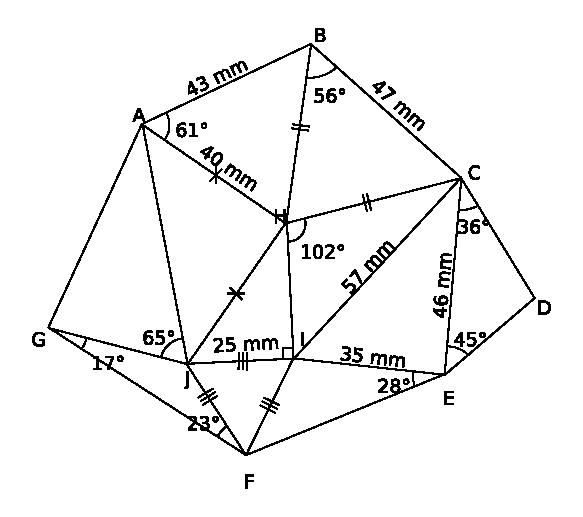
\includegraphics[width=8.3cm]{triangles_many} \end{center}
 \item Construis les triangles suivants : $AGJ$, $AHB$ et $CED$. Que constates-tu ?
 \end{enumerate}
\end{exercice}
